\documentclass[12pt]{article}
\usepackage[a4paper, margin=.30in]{geometry}
\usepackage{graphicx ,
            wrapfig,
            xcolor, 
            enumerate,
            amsmath,fontenc
            }

\newcommand\headerMe[2]{\noindent{}#1\hfill#2}
\renewcommand{\thesection}{\Roman{section}}

\author{Zakaria HAOUZAN}
\date{\today}

\begin{document}
% headers --------------
\headerMe{Matière : Physique-Chimie}{Professeur : Zakaria HAOUZAN}\\
\headerMe{Unité : Introduction }{Établissement : Lycée SKHOR qualifiant}\\
\headerMe{Niveau : 2BAC-SM-X}{Heure : 2H}\\

% ------Content ________
\begin{center}

    \Large{Leçon $N^{\circ} 1 $: \color{red}  Questions qui se posent au chimiste }
\end{center}

%\begin{wrapfigure}[10]{r}{0.5\textwidth}
%    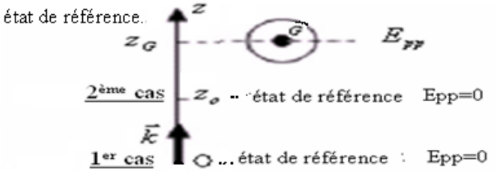
\includegraphics[width=0.5\textwidth]{./img/img00.png}
%\end{wrapfigure}
\section{La chimie :  }
La chimie est une science de la nature expérimentale qui étudie la composition de la matière et ses transformations.

La chimie s'intéresse ainsi aux éléments qui constituent la matière (atomes, ions, etc.), à leurs propriétés et aux liaisons chimiques qui peuvent se créer entre eux.


\section{ Quelques activités du chimiste : }
On a étudié les années précédentes certaines activités du chimiste comme la technique d'extraction et de synthèse et celle
d'analyse chromatographique ...etc .......

Les activités du chimiste sont nombreuses et diversifiées car la chimie est une branche de la science qui étudie la
composition de la matière et ses transformations, elle a un grand rôle dans plusieurs secteurs, elle intervient dans la
fabrication plusieurs produits (médicaments, dentifrice, parfums, peintures, huiles alimentaires, savon, crèmes, colles,
angrais ...etc)

\section{Les questions que se posent au chimiste: }
Plusieurs questions peuvent se poser sur un chimiste parmis lesquelles on peut citer les suivantes: 

\begin{itemize}
	\item Comment augmenter le rendement d'une transformation chimique.
	\item  Quelle est la nature de la transformation étudiée, rapide ou lente? totale ou limitée?
	\item  Quelle est le sens de la transformation, est il direct ou inverse?
	\item Comment contrôler l'évolution d'un système chimique? et plusieurs autres questions qui dépendent de la nature de la recherche chimiste.

\end{itemize}

Par exemple Archimède s'est posé plusieurs questions sur la couronne du roi :
\begin{itemize}
	\item Est-ce la couronne est en or pure ?
	\item Contient-elle un autre métal ?
	\item Le volume de la couronne est il égal au volume de la quantité d'or pure ayant la même masse que la couronne?
	\item Comment déterminer le volume de la couronne ?
	\item Finalement Archimède a constaté que lorsqu'on immerge la couronne dans l'eau, le volume de l'eau déplacée est égale à celui de la
couronne, ce qui lui a permet de déterminer le volume de la couronne et de savoir qu'elle n'était pas en or pure.  
\end{itemize}
\begin{figure}[h!]
\begin{center}
	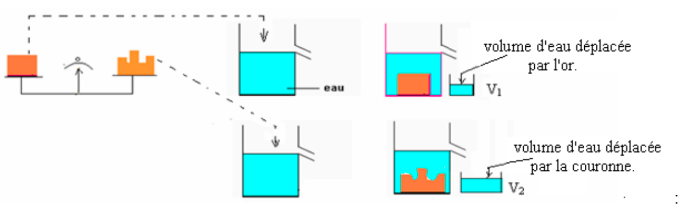
\includegraphics[width=0.8\textwidth]{./chimiste.png}
\end{center}
\end{figure}
Malgré qu'ils ont la même masse, la couronne avait un volume supérieur à celui de l'or pure ayant même masse que celle de la
couronne donc elle n'était pas en or pure, elle contenait un autre métal: l'argent qui a une masse volumique
$10,5g/cm^3$ inférieure à celle de l'or qui est : $19,3g/cm^3$

donc la couronne n'était pas en or pure.

Rappelons quelques notions acquises et qui sont en relation avec les mesures effectués par le chimiste.



\section{Rappel de quelques notions acquises utilisées dans les mesures effectuées par le chimiste:}
\subsection{La quantité de matière:}
La quantité de matière d'un échantillon est le nombre de moles que contient cet échantillon. C'est une grandeur notée n ; son unité
est la mole (mol) ,elle est donnée par l'une des relations suivantes:
 
$n = \frac{N}{N_A}$ ; $n = \frac{m}{M}$ ; $n = \frac{V}{V_M}$ ; $n = C.V$ ; $n = \frac{P.V}{R.T}$ 

\subsection{La masse volumique:}
La masse volumique d'un corps solide liquide ou gazeux est le quotient de sa masse par son volume: $\rho = \frac{m}{V}$

L'unité de la masse volumique dans le système international est : kg/m3 , mais on utilise couramment: g/cm3
.

Exemple masse volumique de l'aluminium: $\rho = 2.7g/cm^3 = \frac{2,7.10^{-3}Kg}{10^{-6}m^3} = 2700 Kg/m^3$

\subsection{ La densité:}
La densité d'un corps solide ou liquide: $d = \frac{\rho}{\rho_{eau}}$, pour les gaz $d = \frac{M}{29}.$

Remarque : la relation $n=\frac{m}{M}$ s'écrit : $n = \frac{m}{M} = \frac{\rho.V}{M} = \frac{\rho_{eau}dV}{M}$

\subsection{Relation de dilution d'une solution: }
Soit V le volume de la solution concentrée et C sa concentration, et soit C' la concentration de la solution diluée et V' son volume.

si $V_e$ est le volume de l'eau ajoutée, on a: $V' = V+V_{e}$

La quantité de matière est la même dans les deux solutions : n = n' donc CV=CV'  C'est la relation de dilution

Le facteur de dilution: $F= \frac{C}{C'} = \frac{V'}{V}$

\end{document}

